\chapter{傅里叶变换}
这一章我们将会学习非常有用的\textbf{傅里叶级数}(Fourier Series)和\textbf{傅里叶变换}(Fourier Transform)。
傅里叶级数和傅里叶变换在数论、组合数学、信号处理、概率论、统计学、密码学、声学、光学等领域都有着广泛的应用。


\section{傅里叶级数}
\label{sec:fourier_series}
\subsection{傅里叶级数的引入}
\label{subsec:fourier_series}
Fourier曾试图解决一个问题,在此过程中发展了傅里叶级数的概念.此问题处理长度为$\ell$的一维均匀棒的热传播过程,即
给定初始温度分布,求解在$t$时刻,$x$处的温度,$T(x,t)$.该温度场满足微分方程
$$
\frac{\partial^2}{\partial x^2} T(x,t) = \frac{\partial}{\partial t} T(x,t), \quad  T(0,t) = T(\ell,t) = 0 .  
$$
该微分方程的一特殊解可以由分离变量法得到,具体方法后面会学习.令$T(x,t) = f(x) g(t)$,代入该方程有
$$
  f''(x) g(t) = f(x) g'(t) ,
$$
两边同除以$f(x)g(t)$得到
$$
\frac{f''(x)}{f(x)} = \frac{g'(t)}{g(t)}   .
$$
由于左式是与$t$无关的,而右边是与$x$无关的,于是唯一可能相等的情况为二者皆为同一个常数$c$.
这时候若$c>0$,可知$\lim_{t\to \infty} g(t) = \infty$,因此我们令$c=-k^2$.
那么可以知道
$$
f(x) =  A \sin{k x} + B \cos{k x},    
$$
由边界条件确定$B = 0$,且$k = \frac{n\pi}{\ell}$.求解$g(t)$得 $g(t) = e^{-k^2 t}$.
该方程的解可以表示为
$$
T(x,t) = A \sin{\left( \frac{n\pi}{\ell} x \right)} e^{-\frac{n^2\pi^2}{\ell^2} t}  
$$
其中$A$由其他条件确定.
可以知道$t=0$时,$T$为一个正弦函数,节点数由$n$决定.但是,更普遍的情况是起始时刻的温度分布并不是正弦函数.
那该如何决定稍后某时刻$t$的分布呢?傅里叶发现我们并不需要对此问题反反复复求解.
对于线性微分方程可以知道若$T_1(x,t)$和$T_2(x,t)$满足微分方程
$$
    \frac{\partial^2}{\partial x^2} T(x,t) = \frac{\partial}{\partial t} T(x,t)
$$
那么二者的任意线性组合
$$
T_3 = \alpha T_1  + \beta T_2  
$$
也是其解.
傅里叶得到结论,对于任意一种光滑的温度分布,其解总可以写成一系列有着不同振幅和模式的正弦函数的线性叠加,即
$$
  T(x,t) = \sum_{n=1}^{\infty} A_n \sin {\left( \frac{n\pi}{\ell} x \right)} e^{-\frac{n^2\pi^2}{\ell^2} t} .     
$$
若初始温度分布函数为$f(x) = T(x,0)$,那么
$$
  f(x) =      \sum_{n=1}^{\infty} A_n \sin {\left( \frac{n\pi}{\ell} x \right)}
$$
上式什么样的函数可以表示为正弦和余弦函数的叠加呢?每个模式的振幅$A_n$该如何计算呢?
这就利用了正余弦函数的特征.

记
\begin{equation}
  \braket{f|g} = \int_0^{2\pi} f^{*}(x) g(x) dx\,,
\end{equation}

可以验证
$$
\braket{\sin{ n x }|\sin{m x }}  =  \braket{\cos{ n x }|\cos {m x }}  =  \delta_{mn}\pi  \; (m\neq 0, n\neq 0)
$$

$$
\braket{\sin{ n x }|\cos{m x }}  =  0
$$
将上式代入,注意修改积分变量上下限可以得到振幅系数
\begin{equation}
  A_n = \frac{2}{\ell} \int_0^{\ell} f(x) \sin{ \left( \frac{n\pi}{\ell} x \right) } dx 
\end{equation}
$A_n$称为傅里叶级数的\textbf{系数}.若所有系数都求得后,我们就得到了$f(x)$.原则上,所有的平滑的单值函数并没有什么问题,
但似乎缺乏数学的严谨.自然,越多的级数项对函数的逼近也就越好.

\subsection{傅里叶定理}
\label{subsec:fourier_theorem}
对于任意一个以$2\ell$为周期的函数,
$$
   f(x + 2\ell) = f(x),  
$$
我们可以通过三角函数族进行级数展开
\begin{equation}
  f(x) = \frac{a_0}{2} + \sum_{n=1}^{\infty} \left[ a_n \cos{ \frac{n\pi}{\ell} x } + b_n \sin{ \frac{n\pi}{\ell} x } \right] 
\end{equation}
利用三角函数族的正交性,可以得到展开系数
\begin{align}
  a_n = \frac{1}{\ell} \int_{-\ell}^{\ell} f(x) \cos {  \left( \frac{n\pi}{\ell} x \right) } dx
  \\
  b_n = \frac{1}{\ell} \int_{-\ell}^{\ell} f(x) \sin {  \left( \frac{n\pi}{\ell} x \right) } dx
\end{align}
这里的积分上下限为一个周期$2\ell$,也可以为$[0,2\ell]$.
上述傅里叶级数展开的成立条件被称为\textbf{狄里希利条件} (Dirichlet conditions),即$f(x)$在$\left[-\ell, \ell\right]$区间内只有有限个间断点,且每个周期内有有限个极值点.满足
这两个条件的函数称为\textbf{分段平常}.
满足狄里希利条件的函数$f(x)$在点$x_0$处间断,那么其傅里叶级数在此点的值为该函数左右值的算术平均
\begin{equation}
  \textrm{级数和}(x_0) = \lim_{\epsilon \to 0} \half \left[
     f(x_0 + \epsilon) + f(x_0  - \epsilon) \right]
\end{equation}

对于奇函数和偶函数的傅里叶展开,不难发现,奇函数的展开为

\begin{equation}
  f(x) = \sum_{n=1}^{\infty} b_n \sin {  \left( \frac{n\pi}{\ell} x \right) }
\end{equation}
称为\textbf{傅里叶正弦级数}.
而偶函数的展开为
\begin{equation}
  f(x) = \frac{a_0}{2} + \sum_{n=1}^{\infty}  a_n \cos{  \left( \frac{n\pi}{\ell} x \right) }
\end{equation}
称为\textbf{傅里叶余弦级数}.

对于复指数的展开,不难发现可以写成
\begin{equation}
  f(x) = \sum_{n=-\infty}^{\infty} c_n e^{\imath \frac{n\pi}{\ell} x},
\end{equation}
其中
$c_n = \half(a_n - \imath b_n)$, $c_{-n} = \half (a_n + \imath b_n)$, $n>0$, $c_0 = \half a_0$.
写出来为
\begin{equation}
  c_n = \frac{1}{2\ell} \int_{-\ell}^{\ell} f(x) e^{-\imath \frac{n\pi}{\ell} x} dx ,
\end{equation}
尽管$f(x)$是实数,但其傅里叶系数却可能是复数,还可以看出$c_{-n} = c_{n}^*$.
复指数函数族也是正交的
$$
  \braket{ e^{\imath \frac{n\pi}{\ell} x } | e^{\imath \frac{m\pi}{\ell} x } } = 2\ell \delta_{mn} .
$$

\begin{example}
对于锯齿函数
$$  
f(x)= \begin{cases}
  x,   &  0 < x \leq  \ell 
  \\
  x - 2 \ell,   & \ell < x \leq 2\ell
\end{cases}
$$
求其傅里叶级数.
\end{example}
\begin{solution}
不难判定通过解析延拓,该函数为奇函数,根据傅里叶展开系数公式,可以得
\begin{align}
b_n &=   \frac{1}{\ell} \int_{0}^{2\ell} f(x) \sin {  \left( \frac{n\pi}{\ell} x \right) } dx \nonumber
\\
&= \frac{1}{\ell} \int_{0}^{\ell} x  \sin {  \left( \frac{n\pi}{\ell} x \right) } dx \nonumber
  % \\ & \quad 
  +
 \frac{1}{\ell} \int_{\ell}^{2\ell} (x - 2\ell) \sin {  \left( \frac{n\pi}{\ell} x \right) } dx \nonumber
 \\ 
 &= \frac{2}{\ell} \int_{0}^{2\ell} x \sin {  \left( \frac{n\pi}{\ell} x \right) } dx \nonumber
%  \\ & \quad 
 -2 \int_{\ell}^{2\ell}   \sin {  \left( \frac{n\pi}{\ell} x \right) } dx \nonumber
 \\
 & = \frac{2\ell}{n\pi} (-1)^{n+1}  \nonumber
%  \\
%  & = \frac{2}{n\pi}  \left[ (-1)^{n+1} (\ell -1)  -1 \right] , \nonumber
\end{align}
因此,该级数为
\begin{align}
f(x) &=  \sum_{n=1}^{\infty} \frac{2 \ell }{n\pi} (-1)^{n+1} \sin {  \left( \frac{n\pi}{\ell} x \right) }  \nonumber
\\
 & =\frac{2\ell}{\pi} \left[ \sin{\frac{\pi x}{\ell} } - \frac{1}{2}\sin{\frac{2\pi x}{\ell} } 
  +  \frac{1}{3}\sin{\frac{3\pi x}{\ell} } + \cdots + \frac{(-1)^{n+1}}{n}\sin{\frac{n\pi x}{\ell} }
 \right] \nonumber
.
\end{align}
容易验证
$$
  f(0) = 0; f(\ell) = 0;
$$
当$x=\ell/2$, 
$$
f(\ell/2) = \ell/2 =   \frac{2\ell}{\pi} \left[ 1 - 0 - \frac{1}{3} + \frac{1}{5} - 0 -\frac{1}{7}+ \cdots \right]
$$
因此,我们得到莱布尼兹等式,即以下等式
$$
\frac{\pi}{4} = 1-\frac{1}{3} + \frac{1}{5} - \frac{1}{7} + \cdots = \sum_{n=0} \frac{(-1)^n}{2n + 1} .
$$
上式可以通过等式
$\int_0^1 \frac{d x}{1+x^2}=\left.\tan ^{-1} x\right|_0 ^1=\frac{\pi}{4}$,和被积函数的级数展开验证.
其实,这里的锯齿函数可以直接用$f(x) = x, -\ell < x < \ell$来表示,相应的间断点则被移到$\pm \ell$处.
\end{solution}


\subsection{能量定理}
由函数的复数傅里叶级数展开可以得到
\begin{equation}
  E = \frac{1}{2\ell} \int_{-\ell}^{\ell} dx f(x)^* f(x) 
 = \frac{1}{2\ell} \int_{-\ell}^{\ell} dx  \sum c_n e^{\imath \frac{n\pi}{\ell} x} \sum c_m e^{-\imath \frac{m\pi}{\ell} x}
 = \sum |c_n|^2
\end{equation}
利用前面的等式$c_n = \half(a_n - \imath b_n)$,  $c_{-n} = \half (a_n + \imath b_n)$, $n>0$, $c_0 = \half a_0$ 可得
\begin{equation}
  E = \frac{a_0^2}{4}+\sum_{n=1}^{\infty}\left(\frac{a_n^2}{2}+\frac{b_n^2}{2}\right) .
\end{equation}
称为\textbf{Parseval等式}(Parseval's identity).
其物理意义指的是,一复杂波形分解为许多波幅为$c_n$的正(余)弦波的叠加,该波所携带的总能量为各个成分波强度的求和.
作为习题,证明对于矩形波,
$f(x)=\left\{ \begin{array}{ll}-1, & x<0 \\ +1, &  x>0\end{array}\right.$, 其傅里叶级数为
$$
f(x)=\frac{4}{\pi} \left[  \sin \pi x+\frac{1}{3} \sin 3 \pi+\frac{1}{5 } \sin 5 x+\cdots \right]
$$
可以发现对于矩形波,其对应的能量为$1$,于是我们有
$$
|f(x)|^2=1=\frac{16}{\pi^2}\left[\frac{1}{2} \frac{1}{1^2}+\frac{1}{2} \frac{1}{3^2}+\frac{1}{2} \frac{1}{5^2}+\cdots\right]
$$
即
$$
\sum_{n=0} \frac{1}{(2n+1)^2} = \frac{\pi^2}{8} .
$$
\subsection{傅里叶变换}
\label{subsec:fourier_transform}
前面我们讨论了周期性体系的傅里叶级数展开.现在我们希望研究非周期性函数的傅里叶展开问题.
假设$f(x)$是定义在$-\infty < x < \infty$的实函数,我们依旧对该函数进行傅里叶级数展开,
该级数必须理解为周期$2\ell$扩展至$\infty$的极限情况.
由于三角函数族的变量为
\[
 \frac{n\pi x}{\ell}    
\]
引入非连续变量
\[\omega_n = \frac{n\pi} {\ell}, \quad k = 0,1,2,\cdots
    \]
可知$\omega_n = n \omega_0$, 其中$\omega_0 = \frac{\pi}{\ell}$为基础频率(Fundamental Frequency),
\[\Delta \omega_n = \omega_n - \omega_{n-1} = \omega_0 . \] 
有
\begin{equation}
    f(x) = \lim_{\ell\to \infty} \sum_{n=-\infty}^{\infty} \left[
        c_n e^{\imath \omega_n x}
        % \frac{a_0}{2} + \sum_{n=1}^{\infty} \left( a_n \cos \omega_n x + b_n \sin \omega_n x \right)
    \right]
\end{equation}
其中系数
\begin{equation}
    c_n = \frac{1}{2\ell} \int_{-\ell}^{\ell} f(x) e^{-\imath \omega_n x} dx 
\end{equation}
取$\ell\to \infty$的极限,则
\[
  \sum_n \to  \frac{ \ell}{\pi}  \int d\omega 
\]
傅里叶系数记为$F(\omega)$,
有
\begin{equation}
    f(x) = \int_{-\infty}^{\infty} \frac{d \omega }{2\pi}F(\omega) e^{\imath \omega x}, % \quad F (\omega) \equiv 2\ell c_n
\end{equation}
上式的积分称为\textbf{傅里叶积分}(Fourier integral),是$f(x)$的\textbf{傅里叶变换}(Fourier transform).
其中
\begin{equation}
    F (\omega) \equiv 2\ell c_n = \int_{-\infty}^{\infty} e^{-\imath \omega x} f(x) dx,
\end{equation}
这被称为\textbf{逆傅里叶变换}(inverse Fourier transform).

傅里叶积分存在的条件由\textbf{傅里叶积分定理}判定: 
若函数 $f(x)$ 在区间 $(-\infty, \infty)$ 上满足条件: $(1) f(x)$ 在 任一有限区间上满足狄里希利条件; (2) $f(x)$ 在 $(-\infty, \infty)$ 
上绝对可积 (即 $\int_{-\infty}^{\infty}|f(x)| dx$ 收敛), 则 $f(x)$ 可表示成傅里叶积分, 且
$$
\textrm{傅里叶积分值} = \lim_{\epsilon\to 0} \half \left[ f(x+\epsilon) + f(x-\epsilon) . \right]
$$
% $F (\omega) \equiv 2\ell c_n$.

% \begin{align}
%     a_n =  \lim_{\ell\to \infty} \frac{1}{\ell} \int_{-\ell}^{\ell} f(x) \cos {  \omega_n x  } dx
%     \\
%     b_n = \frac{1}{\ell} \int_{-\ell}^{\ell} f(x) \sin {   \omega_n x } dx
% \end{align}

若采用正余弦展开,

\begin{equation}
    f(x) =\int_{0}^{\infty} A(\omega) \cos {\omega x} d\omega + \int_{0}^{\infty} B(\omega) \sin {\omega x} d\omega
\end{equation}
其中
\begin{equation}
    \left\{\begin{array}{l}
    A(\omega)=\frac{1}{\pi} \int_{-\infty}^{\infty} f(x) \cos \omega x d x, \\
    B(\omega)=\frac{1}{\pi} \int_{-\infty}^{\infty} f(x) \sin \omega x d x .
    \end{array}\right.
\end{equation}

上式还可以写成

\begin{equation}
    f(x)=\int_0^{\infty} C(\omega) \cos [\omega x-\varphi(\omega)] d \omega,
\end{equation}

其中
$$
\begin{gathered}
C(\omega)=\sqrt{[A(\omega)]^2+[B(\omega)]^2} \\
\varphi(\omega)=\arctan [B(\omega) / A(\omega)] .
\end{gathered}
$$
$C(\omega)$ 称为 $f(x)$ 的振幅谱, $\varphi(\omega)$ 称为 $f(x)$ 的相位谱.如果$f(x)$是奇函数或偶函数,
对应的级数为\textbf{傅里叶余弦积分}或\textbf{傅里叶正弦积分}.

复数形式的傅里叶积分可以写成对称的形式,
\begin{equation}
    \begin{aligned}
    f(x) & =\frac{1}{\sqrt{2 \pi}} \int_{-\infty}^{\infty} F(\omega)e^{\imath \omega x} d \omega, \\
    F(\omega) & =\frac{1}{\sqrt{2 \pi}} \int_{-\infty}^{\infty} f(x)\left[e^{\imath \omega x}\right]^* d x .
    \end{aligned}
\end{equation}
并常用符号简写为
$$
F(\omega)=\mathcal{F}[f(x)], \quad f(x)=\mathcal{F}^{-1}[F(\omega)] .
$$
$f(x)$ 和 $F(\omega)$ 分别称为傅里叶变换的\textbf{原函数}和\textbf{像函数}.

\begin{examplebox}{
求以下函数的复数傅里叶变换.
\begin{enumerate}
    \item $f(x) = e^{-\alpha |x|}, \alpha > 0$;
    \item $f(x) = \delta (x)$;
    \item $f(x) = e^{-\alpha x^2}, \alpha > 0$.
\end{enumerate}
}
\begin{enumerate}
    \item 对$x$分段进行处理,利用对称形式的傅里叶变换有
    \begin{align}
        F(\omega) &=
        \sqrt{\frac{1}{2 \pi}} \int_{-\infty}^0 e^{\alpha x+i \omega t} dx \nonumber
        % \\ &
        +
        \sqrt{\frac{1}{2 \pi}} \int_0^{\infty} e^{-\alpha x+i \omega t} dx  \nonumber
        \\
        &= \sqrt{\frac{1}{2 \pi}} \left[\frac{1}{\alpha + \imath \omega } + \frac{1}{\alpha - \imath \omega } \right] \nonumber
        \\
        &= \sqrt{\frac{1}{2 \pi}} \frac{2\alpha}{\alpha^2 + \omega^2}, \nonumber
    \end{align}
    越大的$\alpha$则$f(x)$越窄,集中在$x=0$附近,也就是越局域,而其傅里叶变换则越弥散.当$f(x)$是偶函数时,傅里叶变换的像函数为实函数.

    \item 代入
    \begin{align}
        F(\omega) &=
        \sqrt{\frac{1}{2 \pi}} \int_{-\infty}^{\infty} \delta(x) e^{+\imath \omega x} d x = \sqrt{\frac{1}{2 \pi}} ,
    \end{align}
    $f(x)$无限局域对应的傅里叶变换为无限弥散.

    \item 类似的,  
    \begin{align}
        F(\omega) &=\frac{1}{\sqrt{2 \pi}} \int_{-\infty}^{\infty} e^{-\alpha x^2} e^{\imath \omega x} d x \nonumber
        % \\ &
        % \\
        % & 
        = \frac{ e^{-\omega^2 / 4\alpha }}{\sqrt{2 \pi}} \int_{-\infty}^{\infty} e^{-\alpha  \left( x - \frac{\imath \omega}{2\alpha} \right)^2}  d x
        \nonumber
        % \\ & 
        \\
        & = \frac{ e^{-\omega^2 / 4\alpha }}{\sqrt{2 \pi}} \int_{-\infty - \imath \omega / 2\alpha}^{\infty - \imath \omega / 2\alpha} e^{-\alpha t^2} dt
        \nonumber
        % \\ &
        \\
        & = \frac{ e^{-\omega^2 / 4\alpha }}{\sqrt{2 \pi}} \sqrt{\frac{\pi}{\alpha}} 
        \nonumber
        % \\ &
        \\
            & = \frac{1}{\sqrt{2\alpha}} e^{- \frac{\omega^2}{4\alpha}} \nonumber .
        % \\ &
    \end{align}
    上式用了变量代换$t = x - \imath \omega /2 \alpha$,高斯函数的像函数还是高斯函数.
\end{enumerate}
\end{examplebox}


\subsection{傅里叶变换基本性质}
傅里叶变换满足以下基本性质.假定$f(x)$的傅里叶变换存在,记为$\mathcal{F}[f(x)] = F(\omega)$.

\begin{enumerate}
    \item 导数定理
    \begin{equation}
        \mathcal{F} [f'(x)] = \imath \omega F(\omega)
    \end{equation}

    \item 积分定理
    \begin{equation}
        \mathcal{F} [ \int^{x} f(x) dx ] = \frac{1}{\imath \omega} F(\omega)
    \end{equation}

    \item 相似性定理
    \begin{equation}
        \mathcal{F} [ f(ax) ] = \frac{1}{a} F(\frac{\omega}{a}),
    \end{equation}
    \item 延迟定理
    \begin{equation}
        \mathcal{F} [ f(x - x_0 ) ] = e^{-\imath \omega x_0} F(\omega),
    \end{equation}
    \item 位移定理
    \begin{equation}
        \mathcal{F} [ e^{\imath \omega x_0} f(x) ] = f(\omega - \omega_0),
    \end{equation}
    \item 卷积定理, 如果
    \[
        \mathcal{F} [f_1(x)] =  F_1(\omega), \mathcal{F} [f_2(x)] =  F_2(\omega), 
    \]
    有
    \begin{equation}
        \mathcal{F} [f_1(x)\star f_2(x) ] = F_1(\omega) F_2(\omega).
    \end{equation}
    其中 $f_1(x) \star f_2(x)=\int_{-\infty}^{\infty} f_1(\alpha) f_2(\alpha-x) d \alpha$ 称为 $f_1(x)$ 与 $f_2(x)$ 的卷积.
\end{enumerate}

\subsection{高维傅里叶变换}

二维连续函数 $f(x, y)$ 的傅里叶变换定义如下:
设 $f(x, y)$ 是两个独立变量 $x, y$ 的函数, 且在 $\pm \infty$ 上绝对可 积, 则定义积分
$$
F\left(k_1, k_2\right)=\frac{1}{2 \pi} \int_{-\infty}^{\infty} \int_{-\infty}^{\infty} f(x, y) e^{-\imath\left(k_1 x+k_2 y\right)} d x d y
$$
为二维连续函数 $f(x, y)$ 的傅里叶变换, 并定义
$$
f(x, y)=\int_{-\infty}^{\infty} \int_{-\infty}^{\infty} F\left(k_1, k_2\right) e^{\imath\left(k_1 x+k_2 y\right)} d k_1 d k_2
$$
为 $F\left(k_1, k_2\right)$ 的逆变换.
$f(x, y)$ 和 $F\left(k_1, k_2\right)$ 称为傅里叶变换对.

\begin{examplebox}{
    求函数 $f(x, y)= \begin{cases}A, & |x| \leq X,|y| \leq Y \\ 0, & |x|>X,|y|>Y\end{cases}$ 的傅里叶变换 (矩孔费琅和夫衍射).
}
由傅里叶变换关系
$$
F\left(k_1, k_2\right)=\frac{1}{(2 \pi)^2} \int_{-\infty}^{\infty} \int_{-\infty}^{\infty} f(x, y) e^{-i\left(k_1 x+k_2 y\right)} d x d y
$$
有
$$
\begin{aligned}
F\left(k_1, k_2\right) & =\frac{A}{2 \pi} \int_X^X e^{-i k_1 x} d x \int_Y^X e^{-i k_2 y} d y \\
& =\left.\left.\frac{A}{2 \pi} \frac{1}{-i k_1} e^{-i k_1 x}\right|_{-X} ^X \frac{1}{-i k_2} e^{-i k_2 y}\right|_{-Y} ^Y \\
& =\frac{2A}{\pi} \frac{1}{i 2 k_1}\left(e^{i k_1 X}-e^{-i k_1 X}\right) \frac{1}{i 2 k_2}\left(e^{i k_2 Y}-e^{-i k_2 Y}\right) \\
& =\frac{2A X Y}{\pi} \frac{\sin \left(k_1 X\right)}{k_1 X} \frac{\sin \left(k_2 Y\right)}{k_2 Y}
\end{aligned}
$$
\end{examplebox}

对于三维情况,$\vec{k}=\left(k_1, k_2, k_3\right), \vec{r}=(x, y, z)$,
\begin{equation}
    F(\vec{k})=\frac{1}{(2 \pi)^3} \iiint_{-\infty}^{\infty} f(\vec{r}) e^{-\imath  \vec{k} \cdot \vec{r}} d^3 \vec{r} \\
\end{equation}
或者
\begin{equation}
    F\left(k_1, k_2, k_3\right)=\frac{1}{(2 \pi)^3} \iiint_{\infty}^{\infty} f(x, y, z) e^{-\imath\left(k_1 x+k_2 y+k_3 z\right)} d x d y d z 
\end{equation}
逆变换为
\begin{equation}
     f(\vec{r})=\iiint_{-\infty}^{\infty} F(k) e^{\imath \vec{k} \cdot \vec{r}} d^3 \vec{k} 
\end{equation}  
或
\begin{equation}
f(x, y, z)=\iiint_{-\infty}^{\infty} F\left(k_1, k_2, k_3\right) e^{\imath\left(k_1 x+k_2 y+k_3 z\right)} d k_1 d k_2 d k_3 
\end{equation} 
\subsection{$\delta$函数}
\label{sub:delta_function}

\subsubsection{$\delta$函数的概念}

物理学常常要研究一个物理量在空间或时间中分布的密度, 例如质量密度 (通常简称为密度)、电荷密度、每单位时间传递的动量 (即力) 等等. 但是物 理学又常常运用质点、点电荷、瞬时力等抽象模型, 它们不是连续分布于空间 或时间中, 而是集中在空间的某一点或时间的某一瞬时. 它们的密度又该如何 描述呢?
我们知道, 若质量 $m$ 均匀分布在长为 $l$ 的线段 $[-l / 2, l / 2]$ 上, 则其线密 度 $\rho_l(x)$ 可表为
$$
\rho_l(x)=\left\{\begin{array}{ll}
0 & (|x|>l / 2), \\
m / l & (|x| \leqslant l / 2),
\end{array} \text { 即 } \rho_l(x)=\frac{m}{l} \operatorname{rect}\left(\frac{x}{l}\right) .\right.
$$
将 $\rho_l(x)$ 对 $x$ 积分, 则得到总质量
$$
\int_{-\infty}^{\infty} \rho_l(x) d x=\int_{-\frac{l}{2}}^{\frac{l}{2}} \frac{m}{l} \mathrm{~d} x=m
$$

如果让上述线段的长度 $l \rightarrow 0$, 我们将得到位于坐标原点质量为 $m$ 的质点, 而线密度函数就成为质点的线密度函数. 将它记为 $\rho(x)$, 则
$$
\lim _{l \rightarrow 0} \int_{-\infty}^{\infty} \rho_l(x) d x=\int_{-\infty}^{\infty} \rho(x) d x=m .
$$
若不求积分而先取极限, 则有
$$
\rho(x)=\lim _{l \rightarrow 0} \rho_l(x)=\lim _{l \rightarrow 0} \frac{m}{l} \operatorname{rect}\left(\frac{x}{l}\right)= \begin{cases}0 & (x \neq 0), \\ \infty & (x=0) .\end{cases}
$$

由此可以看出质点线密度分布函数的直观图像, 它在 $x=0$ 处为 $\infty$, 在 $x \neq$ 0 处为零. 它的积分为 $m$.
对于质点、点电荷、瞬时力这类集中于空间某一点或时间的某一瞬时的抽 象模型, 在物理学中引人 $\delta$ 函数以描述其密度:
$$
\begin{gathered}
\delta(x)= \begin{cases}0 & (x \neq 0), \\
\infty & (x=0) ;\end{cases} \\
\int_a^b \delta(x) d x= \begin{cases}0 & (\text{其他情况}), \\
1 & (a<0<b) .\end{cases}
\end{gathered}
$$
\subsubsection{$\delta$函数的性质}
$\delta$函数的很多性质可以用在实际的计算中,方便实用. 首先它是满足积分为单位1.
$$
\int_{-\infty}^{\infty} \delta(x) d x=1
$$

并且作为被积函数的乘积因子,它具有挑选性特点

$$
\int_{-\infty}^{\infty} f(x) \delta(x-a) d x=f(a).
$$

$\delta(x)$ 是偶函数, 它的导数是奇函数,
$$
\begin{gathered}
\delta(-x)=\delta(x), \\
\delta^{\prime}(-x)=-\delta^{\prime}(x) .
\end{gathered}
$$

对于变量为函数的情况,有
\begin{equation}
    \delta[\varphi(x)]=\sum_k \frac{\delta\left(x-x_k\right)}{\left|\varphi^{\prime}\left(x_k\right)\right|}
\end{equation}
其中$x_k(k=1,2,3, \cdots)$是
$\varphi(x)=0$ 的实根.
特例包括
\begin{equation}
    \begin{gathered}
    \delta(a x)=\frac{\delta(x)}{|a|}, \\
    \delta\left(x^2-a^2\right)=\frac{\delta(x+a)+\delta(x-a)}{2|a|}=\frac{\delta(x+a)+\delta(x-a)}{2|x|} .
    \end{gathered}
\end{equation}

$\delta$函数是一种广义函数,常常可以看作是以下函数的极限.
\begin{equation}
    \begin{aligned}
    & \delta(x)=\lim _{l \rightarrow 0} \frac{1}{l} \operatorname{rect}\left(\frac{x}{l}\right), \\
    & \delta(x)=\lim _{K \rightarrow \infty} \frac{1}{\pi} \frac{\sin K x}{x}, \\
    & \delta(x)=\lim _{\varepsilon \rightarrow 0} \frac{1}{\pi} \frac{\varepsilon}{\varepsilon^2+x^2} .
    \end{aligned}
\end{equation}

\subsubsection{$\delta$ 函数的傅里叶变换}





\subsection{傅里叶变换}
\label{subsec:fourier_transform}
前面我们讨论了周期性体系的傅里叶级数展开。现在我们希望研究非周期性函数的傅里叶展开问题。
假设$f(x)$是定义在$-\infty < x < \infty$的实函数,我们依旧对该函数进行傅里叶级数展开,
该级数必须理解为周期$2\ell$扩展至$\infty$的极限情况。
由于三角函数族的变量为
\[
 \frac{n\pi x}{\ell}    
\]
引入非连续变量
\[\omega_n = \frac{n\pi} {\ell}, \quad k = 0,1,2,\cdots
    \]
可知$\omega_n = n \omega_0$, 其中$\omega_0 = \frac{\pi}{\ell}$为基础频率(Fundamental Frequency),
\[\Delta \omega_n = \omega_n - \omega_{n-1} = \omega_0 \textrm{。} \] 
有
\begin{equation}
    f(x) = \lim_{\ell\to \infty} \sum_{n=-\infty}^{\infty} \left[
        c_n e^{\imath \omega_n x}
        % \frac{a_0}{2} + \sum_{n=1}^{\infty} \left( a_n \cos \omega_n x + b_n \sin \omega_n x \right)
    \right]
\end{equation}
其中系数
\begin{equation}
    c_n = \frac{1}{2\ell} \int_{-\ell}^{\ell} f(x) e^{-\imath \omega_n x} dx 
\end{equation}
取$\ell\to \infty$的极限,则
\[
  \sum_n \to  \frac{ \ell}{\pi}  \int d\omega 
\]
傅里叶系数记为$F(\omega)$,
有
\begin{equation}
    f(x) = \int_{-\infty}^{\infty} \frac{d \omega }{2\pi}F(\omega) e^{\imath \omega x}, % \quad F (\omega) \equiv 2\ell c_n
\end{equation}
上式的积分称为\textbf{傅里叶积分}(Fourier integral),是$f(x)$的\textbf{傅里叶变换}(Fourier transform)。
其中
\begin{equation}
    F (\omega) \equiv 2\ell c_n = \int_{-\infty}^{\infty} e^{-\imath \omega x} f(x) dx,
\end{equation}
这被称为\textbf{逆傅里叶变换}(inverse Fourier transform)。

傅里叶积分存在的条件由\textbf{傅里叶积分定理}判定: 
若函数 $f(x)$ 在区间 $(-\infty, \infty)$ 上满足条件: $(1) f(x)$ 在 任一有限区间上满足狄里希利条件; (2) $f(x)$ 在 $(-\infty, \infty)$ 
上绝对可积 (即 $\int_{-\infty}^{\infty}|f(x)| dx$ 收敛), 则 $f(x)$ 可表示成傅里叶积分, 且
$$
\textrm{傅里叶积分值} = \lim_{\epsilon\to 0} \half \left[ f(x+\epsilon) + f(x-\epsilon) \textrm{。} \right]
$$
% $F (\omega) \equiv 2\ell c_n$。

% \begin{align}
%     a_n =  \lim_{\ell\to \infty} \frac{1}{\ell} \int_{-\ell}^{\ell} f(x) \cos {  \omega_n x  } dx
%     \\
%     b_n = \frac{1}{\ell} \int_{-\ell}^{\ell} f(x) \sin {   \omega_n x } dx
% \end{align}

若采用正余弦展开,

\begin{equation}
    f(x) =\int_{0}^{\infty} A(\omega) \cos {\omega x} d\omega + \int_{0}^{\infty} B(\omega) \sin {\omega x} d\omega
\end{equation}
其中
\begin{equation}
    \left\{\begin{array}{l}
    A(\omega)=\frac{1}{\pi} \int_{-\infty}^{\infty} f(x) \cos \omega x d x, \\
    B(\omega)=\frac{1}{\pi} \int_{-\infty}^{\infty} f(x) \sin \omega x d x .
    \end{array}\right.
\end{equation}

上式还可以写成

\begin{equation}
    f(x)=\int_0^{\infty} C(\omega) \cos [\omega x-\varphi(\omega)] d \omega,
\end{equation}

其中
$$
\begin{gathered}
C(\omega)=\sqrt{[A(\omega)]^2+[B(\omega)]^2} \\
\varphi(\omega)=\arctan [B(\omega) / A(\omega)] .
\end{gathered}
$$
$C(\omega)$ 称为 $f(x)$ 的振幅谱, $\varphi(\omega)$ 称为 $f(x)$ 的相位谱。如果$f(x)$是奇函数或偶函数,
对应的级数为\textbf{傅里叶余弦积分}或\textbf{傅里叶正弦积分}。

复数形式的傅里叶积分可以写成对称的形式,
\begin{equation}
    \begin{aligned}
    f(x) & =\frac{1}{\sqrt{2 \pi}} \int_{-\infty}^{\infty} F(\omega)e^{\imath \omega x} d \omega, \\
    F(\omega) & =\frac{1}{\sqrt{2 \pi}} \int_{-\infty}^{\infty} f(x)\left[e^{\imath \omega x}\right]^* d x .
    \end{aligned}
\end{equation}
并常用符号简写为
$$
F(\omega)=\mathcal{F}[f(x)], \quad f(x)=\mathcal{F}^{-1}[F(\omega)] \textrm{。}
$$
$f(x)$ 和 $F(\omega)$ 分别称为傅里叶变换的\textbf{原函数}和\textbf{像函数}。

\begin{examplebox}{
求以下函数的复数傅里叶变换。
\begin{enumerate}
    \item $f(x) = e^{-\alpha |x|}, \alpha > 0$;
    \item $f(x) = \delta (x)$;
    \item $f(x) = e^{-\alpha x^2}, \alpha > 0$。
\end{enumerate}
}
\begin{enumerate}
    \item 对$x$分段进行处理,利用对称形式的傅里叶变换有
    \begin{align}
        F(\omega) &=
        \sqrt{\frac{1}{2 \pi}} \int_{-\infty}^0 e^{\alpha x+i \omega t} dx \nonumber
        % \\ &
        +
        \sqrt{\frac{1}{2 \pi}} \int_0^{\infty} e^{-\alpha x+i \omega t} dx  \nonumber
        \\
        &= \sqrt{\frac{1}{2 \pi}} \left[\frac{1}{\alpha + \imath \omega } + \frac{1}{\alpha - \imath \omega } \right] \nonumber
        \\
        &= \sqrt{\frac{1}{2 \pi}} \frac{2\alpha}{\alpha^2 + \omega^2}, \nonumber
    \end{align}
    越大的$\alpha$则$f(x)$越窄,集中在$x=0$附近,也就是越局域,而其傅里叶变换则越弥散。当$f(x)$是偶函数时,傅里叶变换的像函数为实函数。

    \item 代入
    \begin{align}
        F(\omega) &=
        \sqrt{\frac{1}{2 \pi}} \int_{-\infty}^{\infty} \delta(x) e^{+\imath \omega x} d x = \sqrt{\frac{1}{2 \pi}} \textrm{,}
    \end{align}
    $f(x)$无限局域对应的傅里叶变换为无限弥散。

    \item 类似的,  
    \begin{align}
        F(\omega) &=\frac{1}{\sqrt{2 \pi}} \int_{-\infty}^{\infty} e^{-\alpha x^2} e^{\imath \omega x} d x \nonumber
        % \\ &
        % \\
        % & 
        = \frac{ e^{-\omega^2 / 4\alpha }}{\sqrt{2 \pi}} \int_{-\infty}^{\infty} e^{-\alpha  \left( x - \frac{\imath \omega}{2\alpha} \right)^2}  d x
        \nonumber
        % \\ & 
        \\
        & = \frac{ e^{-\omega^2 / 4\alpha }}{\sqrt{2 \pi}} \int_{-\infty - \imath \omega / 2\alpha}^{\infty - \imath \omega / 2\alpha} e^{-\alpha t^2} dt
        \nonumber
        % \\ &
        \\
        & = \frac{ e^{-\omega^2 / 4\alpha }}{\sqrt{2 \pi}} \sqrt{\frac{\pi}{\alpha}} 
        \nonumber
        % \\ &
        \\
            & = \frac{1}{\sqrt{2\alpha}} e^{- \frac{\omega^2}{4\alpha}} \nonumber \textrm{。}
        % \\ &
    \end{align}
    上式用了变量代换$t = x - \imath \omega /2 \alpha$,高斯函数的像函数还是高斯函数。
\end{enumerate}
\end{examplebox}


\subsection{傅里叶变换基本性质}
傅里叶变换满足以下基本性质。假定$f(x)$的傅里叶变换存在,记为$\mathcal{F}[f(x)] = F(\omega)$。

\begin{enumerate}
    \item 导数定理
    \begin{equation}
        \mathcal{F} [f'(x)] = \imath \omega F(\omega)
    \end{equation}

    \item 积分定理
    \begin{equation}
        \mathcal{F} [ \int^{x} f(x) dx ] = \frac{1}{\imath \omega} F(\omega)
    \end{equation}

    \item 相似性定理
    \begin{equation}
        \mathcal{F} [ f(ax) ] = \frac{1}{a} F(\frac{\omega}{a}),
    \end{equation}
    \item 延迟定理
    \begin{equation}
        \mathcal{F} [ f(x - x_0 ) ] = e^{-\imath \omega x_0} F(\omega),
    \end{equation}
    \item 位移定理
    \begin{equation}
        \mathcal{F} [ e^{\imath \omega x_0} f(x) ] = f(\omega - \omega_0),
    \end{equation}
    \item 卷积定理, 如果
    \[
        \mathcal{F} [f_1(x)] =  F_1(\omega), \mathcal{F} [f_2(x)] =  F_2(\omega), 
    \]
    有
    \begin{equation}
        \mathcal{F} [f_1(x)\star f_2(x) ] = F_1(\omega) F_2(\omega).
    \end{equation}
    其中 $f_1(x) \star f_2(x)=\int_{-\infty}^{\infty} f_1(\alpha) f_2(\alpha-x) d \alpha$ 称为 $f_1(x)$ 与 $f_2(x)$ 的卷积。
\end{enumerate}

\subsection{高维傅里叶变换}

二维连续函数 $f(x, y)$ 的傅里叶变换定义如下:
设 $f(x, y)$ 是两个独立变量 $x, y$ 的函数, 且在 $\pm \infty$ 上绝对可 积, 则定义积分
$$
F\left(k_1, k_2\right)=\frac{1}{2 \pi} \int_{-\infty}^{\infty} \int_{-\infty}^{\infty} f(x, y) e^{-\imath\left(k_1 x+k_2 y\right)} d x d y
$$
为二维连续函数 $f(x, y)$ 的傅里叶变换, 并定义
$$
f(x, y)=\int_{-\infty}^{\infty} \int_{-\infty}^{\infty} F\left(k_1, k_2\right) e^{\imath\left(k_1 x+k_2 y\right)} d k_1 d k_2
$$
为 $F\left(k_1, k_2\right)$ 的逆变换。
$f(x, y)$ 和 $F\left(k_1, k_2\right)$ 称为傅里叶变换对。

\begin{examplebox}{
    求函数 $f(x, y)= \begin{cases}A, & |x| \leq X,|y| \leq Y \\ 0, & |x|>X,|y|>Y\end{cases}$ 的傅里叶变换 (矩孔费琅和夫衍射)。
}
由傅里叶变换关系
$$
F\left(k_1, k_2\right)=\frac{1}{(2 \pi)^2} \int_{-\infty}^{\infty} \int_{-\infty}^{\infty} f(x, y) e^{-i\left(k_1 x+k_2 y\right)} d x d y
$$
有
$$
\begin{aligned}
F\left(k_1, k_2\right) & =\frac{A}{2 \pi} \int_X^X e^{-i k_1 x} d x \int_Y^X e^{-i k_2 y} d y \\
& =\left.\left.\frac{A}{2 \pi} \frac{1}{-i k_1} e^{-i k_1 x}\right|_{-X} ^X \frac{1}{-i k_2} e^{-i k_2 y}\right|_{-Y} ^Y \\
& =\frac{2A}{\pi} \frac{1}{i 2 k_1}\left(e^{i k_1 X}-e^{-i k_1 X}\right) \frac{1}{i 2 k_2}\left(e^{i k_2 Y}-e^{-i k_2 Y}\right) \\
& =\frac{2A X Y}{\pi} \frac{\sin \left(k_1 X\right)}{k_1 X} \frac{\sin \left(k_2 Y\right)}{k_2 Y}
\end{aligned}
$$
\end{examplebox}

对于三维情况,$\vec{k}=\left(k_1, k_2, k_3\right), \vec{r}=(x, y, z)$,
\begin{equation}
    F(\vec{k})=\frac{1}{(2 \pi)^3} \iiint_{-\infty}^{\infty} f(\vec{r}) e^{-\imath  \vec{k} \cdot \vec{r}} d^3 \vec{r} \\
\end{equation}
或者
\begin{equation}
    F\left(k_1, k_2, k_3\right)=\frac{1}{(2 \pi)^3} \iiint_{\infty}^{\infty} f(x, y, z) e^{-\imath\left(k_1 x+k_2 y+k_3 z\right)} d x d y d z 
\end{equation}
逆变换为
\begin{equation}
     f(\vec{r})=\iiint_{-\infty}^{\infty} F(k) e^{\imath \vec{k} \cdot \vec{r}} d^3 \vec{k} 
\end{equation}  
或
\begin{equation}
f(x, y, z)=\iiint_{-\infty}^{\infty} F\left(k_1, k_2, k_3\right) e^{\imath\left(k_1 x+k_2 y+k_3 z\right)} d k_1 d k_2 d k_3 
\end{equation} 
% \section{复变函数积分}
% \subsection[定义和性质]{复变函数的积分}
有了复变函数微分的基础,我们现在来讨论积分.复变函数的积分的定义可以同实变函数积分的类比得到.
在复平面上取一个路径$\ell$,起终点为$A(z_0),B(z_n)$,沿着该路径定义了一连续函数$f(z)$,用$n-1$个点$z_1, z_2,\cdot, z_{n-1}$将该路径
$\ell$分成$n$个线段(见图\ref{fig:complex_integral}).函数$f(z)$在线段$z_{k-1}\rightarrow z_{k}$上任意一点$\xi_k$的值乘上线段的长度$\Delta z_k = z_k - z_{k-1}$并求和,即
\begin{equation}
    S_n = \sum_{k=1}^{n} f(\xi_k) (z_{k} - z_{k-1}) .
\end{equation}
\begin{figure}[htbp]
    \centering
    \chapter{定积分的计算}
对于实变函数的定积分,我们已经学会了一些积分技巧,如变量代换,分部积分等.这一章我们将介绍利用留数定理的积分技巧,并介绍以物理学家Richard P. Feynman命名的
特殊技巧.

% \section{留数定理应用}
\subsection{三角函数的积分}
考虑积分区间为$\left[ 0, 2\pi \right]$,被积函数为三角函数有理式的积分
\begin{equation}
    \int_{0}^{2\pi} R(\cos{x}, \sin{x}) dx,
\end{equation}
当实变数 $x$ 从 0 变到 $2 \pi$ 时, 复变数 $z=e^{\imath x}$ 从 $z=1$ 出发沿单位圆 $|z|=1$ 逆时针 走一圈又回到 $z=1$,
实变定积分化为复变回路积分, 就可以应用留数定理了. 至于实变定积分里的 $\cos x, \sin x$ 和 $d x$, 作如下变换:
$$
\cos x=\frac{1}{2}\left(z+z^{-1}\right), \quad \sin x=\frac{1}{2 \imath}\left(z-z^{-1}\right), \quad d x=\frac{1}{\imath z} d z .
$$
于是, 原积分化为
$$
I=\oint_{|z|=1} R\left(\frac{z+z^{-1}}{2}, \frac{z-z^{-1}}{2 \imath}\right) \frac{d z}{\imath z}
$$
利用留数定理即可求得.

\begin{example}
求定积分\[I=\int_0^{2 \pi} \frac{d \theta}{1+a \cos \theta}, \quad|a|<1 \]
\end{example}
\begin{solution}
    根据上面的方法,可得
    \[
        \begin{aligned}
        I & =-\imath \oint_{|z|=1} \frac{d z}{z\left[1+(a / 2)\left(z+z^{-1}\right)\right]} \\
        & =-\imath \frac{2}{a} \oint \frac{d z}{z^2+(2 / a) z+1} .
        \end{aligned}
    \]
    两个极点分别为
    \[
        z_1=-\frac{1+\sqrt{1-a^2}}{a} \quad \text {和} \quad z_2=-\frac{1-\sqrt{1-a^2}}{a}
    \]
    不难看出,$z_1$在单位圆外,$z_2$在单位圆内.积分可以写成
    \[
      \oint \frac{dz}{(z-z_1)(z-z_2)}   
    \]
    留数则为$\frac{1}{z_2 - z_1}$, 利用留数定理可得 
    \[
      I=  -\imath \frac{2}{a} 2\pi\imath \frac{1}{z_2 - z_1} = \frac{2}{\sqrt{1 - a^2}} . 
    \]
\end{solution}



\subsection{积分上下限为$( -\infty, \infty)$}
 考虑如下形式的定积分
 \[
    \int_{-\infty}^{\infty} f(x) dx
 \]
 我们先讨论复变函数 $f(z)$ 在实轴上没有奇点的情况,有奇点的情况后面讨论. 
被积函数在上半平面除有限个奇点外是解析的; 当 $z$ 在上半平面及实轴上 $\to \infty$ 时, 
$z f(z)$ 一致地 $\to 0$.

取如图所示的上半平面的半径为$R$的半圆路径$\ell$.路径积分可以写成两部分的和
\begin{equation}
    \oint_l f(z) d z=\int_{-R}^R f(x) d x+\int_{C_R} f(z) d z .
\end{equation}
根据留数定理,上式等于$2\pi \imath  \sum_j \Res f(z_j)$.
%\input{tikz/semicircle.tex}
\begin{figure}[htb!]
    \centering
    \input{tikz/semicircle.tex}
    \caption{半圆路径.}
    \label{fig:semicircle}
\end{figure}
下面证明上式第二项为零.一般的对于任意$\theta_1 \leq \theta \leq \theta_2$, 
有$\lim_{R\to \infty} zf(z) = 0$,可以证明对于该角度对应的圆弧$C$有,
\begin{equation}
    \lim_{R \rightarrow \infty} \int_C f(z) dz = 0 .
\end{equation}

\[
    \begin{aligned}
    \lim _{R \rightarrow \infty}\left|\int_C f(z) d z\right| \leq \int_{\theta_1}^{\theta_2} \lim _{R \rightarrow \infty}\left|f\left(R e^{i \theta}\right) i R e^{i \theta}\right| & d \theta \\
    & \leq\left(\theta_2-\theta_1\right) \lim _{R \rightarrow \infty}\left|f\left(R e^{i \theta}\right) R e^{i \theta}\right|=0 .
    \end{aligned}
\]
也就是说,
\begin{equation}
    \int_{-R}^R f(x) d x = 2\pi \imath  \sum_{z_j\in \textrm{上半平面}} \Res f(z_j),
\end{equation}

\begin{example}
    计算\[ 
    I = \int_{-\infty}^{\infty} \frac{dx}{1 + x^2}   .
    \]
\end{example}
\begin{solution}
    由$f(z) = \frac{1}{1+ x^2} = \frac{1}{(z-\imath)(z+\imath)}$可知
    其单极点$\pm \imath$,其中$\imath$在上半平面.
    \[
      \Res f(+\imath) = \frac{1}{2\imath}  
    \]
    因此,$I = 2\pi \imath  \frac{1}{2\imath} = \pi$.由于该积分是一个常见积分
    亦可以通过原函数$\arctan(x)$得到.留数定理的还可以计算这样的积分,
    \[
      I\int_{-\infty}^{\infty} \frac{dx}{(1 + x^2)^n} 
    \]
    具体求解过程参考梁昆淼数学物理方法的解.
\end{solution}


 \subsection{带复指数的定积分}
 考虑以下类型的定积分
 \begin{equation}
    I=\int_{-\infty}^{\infty} f(x) e^{\imath m x} d x
\end{equation}
其中,$m$为正实数;$f(z)$在上半平面除有限个奇点外是解析的,且$\lim_{|z|\to \infty} f(z) = 0, 0 \leq arg z \leq \pi$.
我们使用同样的半圆路径,类似的可以通过留数定理将实轴的积分转换为环路积分求得.
为了使用留数定理,我们先需要证明在半圆上的路径积分为零,这里就要用到\textbf{约旦引理}(Jordan lemma
).
即证明
\begin{equation}
    \lim _{R \rightarrow \infty} \int_{C_R} f(z) e^{\imath m z} d z=0 .
\end{equation}
当$R$足够大时,我们有$|f(z)| < \epsilon$.半圆积分
\begin{align}
    I_R&=\int_0^\pi f\left(R e^{\imath \theta}\right) 
    e^{\imath m R \cos \theta- m R \sin \theta} \imath R e^{\imath \theta} d \theta
    \\
    &\leq \epsilon R \int_0^\pi e^{-m R \sin \theta} d \theta=2 \epsilon R \int_0^{\pi / 2} e^{-m R \sin \theta} d \theta,
\end{align}
可以发现在$\left[ 0, \pi/2\right]$时,
\begin{equation}
    \frac{2}{\pi}\theta \leq \sin{\theta},
\end{equation}
于是有
\begin{equation}
    I_R \leq 2 \epsilon R \int_0^{\pi / 2} e^{-2 m R \theta / \pi} d \theta=2 \epsilon R \frac{1-e^{-m R}}{2 m R / \pi}<\frac{\pi}{m} \epsilon
\end{equation}
即
\begin{equation}
    \lim_{R\to \infty} I_R = 0.
\end{equation}
回到定积分$I$,可以得
\begin{equation}
    \label{eq:complex_exponential_integral}
    I=\int_{-\infty}^{\infty} f(x) e^{ \imath m x} d x = 2\pi \imath \sum_{z_j \in \text{上半平面}} \Res e^{\imath m z_j} f(z_j)
\end{equation}

对于以下类型的积分,可以利用上述结论.如
\begin{equation}
    \int_{0}^{\infty} f(x) \cos {m x} dx, \int_{0}^{\infty} G(x) \sin{m x} dx
\end{equation}
其中,$F(z)$为偶函数,$G(z)$为奇函数,它们在实轴上没有奇点,上半平面上除有限个奇点外解析.
很容易通过$\cos{mx} = \frac{1}{2}\left( e^{\imath m x} + e^{-\imath mx}\right)$等变换得到,即
$$
\begin{aligned}
\int_0^{\infty} F(x) \cos m x d x & =\int_0^{\infty} F(x) \frac{1}{2}\left(e^{\imath m x}+e^{-\imath m x}\right) d x \\
& =\frac{1}{2} \int_0^{\infty} F(x) e^{\imath m x} d x+\frac{1}{2} \int_0^{\infty} F(x) e^{-\imath m x} d x 
\\
& = \frac{1}{2} \int_{-\infty}^{\infty} F(x) e^{\imath m x} d x. 
\end{aligned}
$$

\begin{example}
计算 $\int_0^{\infty} \frac{\cos m x}{x^2+a^2} d x$.
\end{example}
\begin{solution}
偶函数$F(z) e^{\imath m z}=\frac{1}{z^2+a^2} e^{\imath m z}$ 有两个单极点 $\pm a \imath$, 其中 $+a \imath$ 在上半平面. 而 $e^{\imath m z} /\left(z^2+a^2\right)$ 在单极点 $+a \imath$ 的留数为
    $$
    \lim _{z \rightarrow a \imath}\left[(z-a \imath) \frac{e^{\imath m z}}{z^2+a^2}\right]=\lim _{z \rightarrow a \imath}\left[\frac{e^{\imath m z}}{z+a \imath}\right]=\frac{e^{-m a}}{2 a \imath}
    $$
    应用\eqref{eq:complex_exponential_integral},
    $$
    \int_0^{\infty} \frac{\cos m x}{x^2+a^2} d x=\pi \imath \frac{e^{-m a}}{2 a \imath}=\frac{\pi}{2 a} e^{-m a}.
    $$
\end{solution}
\section{Feynman技巧}
我们将讨论下面几个计算定积分的技巧.

\subsection{复变量代换}
以一个例子说明复变量代换的方法.求解定积分
\[
    I =  \int_0^{\infty} e^{-a x} \cos b x d x \\
\]
利用$\cos{bx} = \frac{1}{2}\left( e^{\imath b x} + e^{-\imath bx}\right)$
\[    \begin{aligned}
    I= & \frac{1}{2} \int_{0}^{\infty} \left(e^{-(a-\imath b) x} + e^{-(a + \imath b) x} \right)  d x \\
    = & \frac{1}{2} \left( \frac{1}{a-\imath b} +  \frac{1}{a+\imath b} \right)\\
    = & \frac{a}{a^2+b^2}
\end{aligned}
\]

\subsection{参数微分}
求解定积分
\[
    I =  \int_0^{\infty} x e^{-a x} \cos b x d x \\
\]
我们令
\[
  S(a) =   \int_0^{\infty} e^{-a x} \cos b x d x 
\]
已知 $S(a) = \frac{a}{a^2+b^2}$,通过对$S(a)$对$a$的求导得到
\[
    I = - S'(a)  = \frac{a^2 - b^2}{(a^2 +b^2)^2}    
\]
对于一般的含参数的微分,我们有
\begin{equation}
    \begin{aligned}
    \frac{d}{d \alpha} \int_{x_1(\alpha)}^{x_2(\alpha)} f(x, \alpha) d x= & \int_{x_1}^{x_2} \frac{\partial}{\partial \alpha} f(x, \alpha) d x \\
    & \left[\frac{d x_2(\alpha)}{d \alpha} \right] f(x_2, \alpha)- 
    \left[\frac{d x_1(\alpha)}{d \alpha}\right] f(x_1, \alpha)
    \end{aligned}
\end{equation}

\subsection{被积函数添加函数因子}
求解定积分
\[
    I =  \int_0^{\infty} \frac{\sin{x}}{x} d x 
\]
可以通过乘以一个函数因子$e^{-a x}$来构造参数函数
\[
 S(a) =     \int_0^{\infty}  e^{-a x} \frac{\sin{x}}{x} d x 
\]
这样我们有
\[
  S'(a) = -  \int_0^{\infty}  e^{-a x} \sin{x} d x  = \frac{1}{1+a^2}
\]
对于$a \to \infty$, 有 $S(\infty) = 0$.
而$\frac{1}{1+x^2}$的原函数为$\arctan{x}$,因此
\[S(a) = - \arctan{a} + C\]
可确定$C = \frac{\pi}{2}$,因此我们有$S(a) = \frac{\pi}{2} - \arctan{\alpha}$.
因此,
\[
  I = S(0) = \frac{\pi}{2} .    
\]
该结果我们已通过留数定理求得.
\section{积分求解实例}

\begin{itemize}
    \item 计算定积分 
    $$
    I=\int_0^{\infty} x^{\alpha-1} \frac{1}{1+x} d x \quad(0<\alpha<1).
    $$

    解 将被积函数 $x^{\alpha-1} /(1+x)$ 从实轴延拓到复数 $z$ 平面得到 
    $f(z)=z^{\alpha-1} /(1+z)$. 由于 $f(z)$ 含 有 $z^{\alpha-1}$ ,
    而 $\alpha$ 不是整数,所以 $f(z)$ 是多值函数, 它有两个支点:原点和无限远点. 
    $z$ 每绕原点或 无限远点一圈, 辐角增加 $2 \pi, z^{\alpha-1}$ 多出因子 
    $e^{\imath 2 \pi(\alpha-1)}$ 亦即 $e^{\imath 2 \pi \alpha}$,
     从而 $f(z)$ 也多出这么一个 因子.
    从原点沿着正实轴直至无限远作割线.   
    
    $$
\oint_l f(z) d z=\int_{\epsilon}^R \frac{x^{\alpha-1}}{1+x} d x+\int_{C_R} f(z) d z+\int_R^{\epsilon} \frac{x^{\alpha-1} e^{\imath 2 \pi \alpha}}{1+x} d x+\int_{C_{\epsilon}} f(z) d z .
$$
令 $R \rightarrow \infty, \epsilon \rightarrow 0$.
 上式左边按照留数定理应为 $2 \pi i\{f(z)$ 在有限远各奇点留数之和\}
  右边第一个积分成为所求的 $I$, 第三个积分则成为 $-e^{\imath 2 \pi \alpha} I$. 
  可以证明第 二个和第四个积分则成为零. 事实上,
  $$
\begin{aligned}
\left|\int_{C_R} \frac{z^{\alpha-1}}{1+z} d z\right| & =\left|\int_{C_R} \frac{z^\alpha}{1+z} \frac{d z}{z}\right| \leqslant \max _{\left(C_R \text { 上 }\right)}\left|\frac{z^\alpha}{1+z}\right| \frac{\int|d z|}{|z|} \\
= & \max \frac{R^\alpha}{|1+z|} \cdot \frac{2 \pi R}{R}=2 \pi \max \frac{R^\alpha}{|1+z|} \\
& \sim 2 \pi \frac{1}{R^{1-\alpha} \rightarrow 0} \quad(\text { 于 } R \rightarrow \infty) .
\end{aligned}
$$

$$
\begin{aligned}
\left|\int_{C_{\epsilon}} \frac{z^{\alpha-1}}{1+z} d z\right|= & \left|\int_{C_{\epsilon}} \frac{z^\alpha}{1+z} \frac{d z}{z}\right| \leqslant \max _{\left(C_{\epsilon} \text { 上 }\right)}\left|\frac{z^\alpha}{1+z}\right| \frac{\int|d z|}{|z|} \\
= & \max \frac{\epsilon^\alpha}{|1+z|} \cdot \frac{2 \pi \epsilon}{\epsilon}=2 \pi \max \frac{\epsilon^\alpha}{|1+z|} \\
& \sim 2 \pi \frac{\epsilon^\alpha}{1} \rightarrow 0 \quad(\text { 于 } \epsilon \rightarrow 0) .
\end{aligned}
$$
于是 $\left(1-e^{\imath 2 \pi \alpha}\right) I=2 \pi \imath\{f(z)$ 在有限远各奇点留数之和 $\}$.
$f(z)=z^{\alpha-1}(1+z)^{-1}$ 只有一个单极点 $z_0=-1=e^{\imath \pi}$, 而
$$
\Res f(-1)=\lim _{z \rightarrow-1}[(z+1) f(z)]=\lim _{z \rightarrow-1}\left[z^{\alpha-1}\right]=e^{\imath(\alpha \pi-\pi)}=-e^{\imath \alpha \pi} \text {. }
$$
因此
$$
\begin{aligned}
I & =-\frac{2 \pi \imath e^{\imath \pi \alpha}}{1-e^{\imath 2 \pi \alpha}}=-\frac{2 \pi \imath e^{\imath \pi \alpha}}{e^{\imath \pi \alpha}\left(e^{-\imath \pi \alpha}-e^{\imath \pi \alpha}\right)} \\
& =\frac{2 \pi \imath}{\left(e^{-\imath \pi \alpha}-e^{\imath \pi \alpha}\right)}=\frac{2 \pi \imath}{2 \sin \pi \alpha}=\frac{\pi}{\sin \pi \alpha} .
\end{aligned}
$$

    \item 计算菲涅耳积分(Fresnel integrals)
    $$
    I_1=\int_0^{\infty} \sin \left(x^2\right) \mathrm{d} x \text { 及 } I_2=\int_0^{\infty} \cos \left(x^2\right) \mathrm{d} x \text {. }
    $$

    解 由于 $\sin \left(x^2\right)=\operatorname{Im} e^{\imath x^2}$, 而 $\cos \left(x^2\right)=\operatorname{Re} e^{\imath x^2}$, 所以
$$
I_2+\imath I_1=\int_0^{\infty} e^{\imath x^2} d x .
$$
取图 4-10 所示回路 $l$. 由于 $e^{\mathrm{iz}^2}$ 没有有限远奇点, 所以根据留数定理得
$$
\oint_l e^{\imath z^2} d z=0,
$$
即 $\int_0^R e^{\imath x^2} d x+\int_{C_R} e^{\imath z^2} d z+\int_R^0 e^{\imath\left(\rho e^{\imath \pi / 4}\right)^2} d\left(\rho e^{\imath \pi / 4}\right)=0$,

令 $R \rightarrow \infty$. 第一个积分即所求的 $I_2+\imath I_1$. 第三个积分不难如下算出 :
$$
\begin{aligned}
\lim _{R \rightarrow \infty} \int_R^0 e^{\imath\left(\rho^2 \imath\right)} e^{\imath \pi / 4} d \rho & =\lim _{R \rightarrow \infty}\left(-e^{\imath \pi / 4}\right) \int_0^R e^{-\rho^2} d \rho=-e^{\imath \pi / 4} \int_0^{\infty} e^{-\rho^2} d \rho \\
& =-\frac{\sqrt{\pi}}{2} e^{\imath \pi / 4}=-(1+\imath) \sqrt{\frac{\pi}{8}} .
\end{aligned}
$$
可以证明第二个积分成为零. 为此, 先作一次分部积分,
$$
\int_{C_R} e^{\imath z^2} d z=\left.\frac{e^{\imath z^2}}{2 \imath z}\right|_{z=R} ^{R e^{\imath \pi / 4}}+\int_{C_R} e^{\imath z^2} \frac{\mathrm{d} z}{2 \imath z^2},
$$
其中已积出部分的模
$$
\left|\frac{e^{-R^2}}{2 \imath R e^{\imath \pi / 4}}-\frac{e^{\imath R^2}}{2 \imath R}\right| \leqslant \frac{e^{-R^2}}{2 R}+\frac{1}{2 R} \rightarrow 0 \quad(\text { 于 } R \rightarrow \infty),
$$
未积出部分的模
$$
\begin{aligned}
\left|\int_{C_R} \frac{e^{\imath 2^2}}{2 \imath {z}^2} d z\right| & =\left|\int_{C_R} \frac{e^{-R^2 \sin 2 \varphi+\imath^2 \cos 2 \varphi}}{2 \imath R^2 e^{\imath 2 \varphi}} R e^{\imath \varphi} \imath d \varphi\right| \\
& \leqslant \int_{C_R} \frac{e^{-R^2 \sin 2 \varphi}}{2 R^2} R d \varphi \leqslant \max \left(\frac{e^{-R^2 \sin 2 \varphi}}{2 R}\right) \frac{\pi}{4}
\\
&=\frac{1}{2 R} \frac{\pi}{4} \rightarrow 0 \quad(\text { 于 } R \rightarrow \infty) .
\end{aligned}
$$
于是
$$
\begin{gathered}
I_2+\imath I_1-\sqrt{\frac{\pi}{8}}(1+\imath)=0, \\
I_1=\sqrt{\frac{\pi}{8}}, \quad I_2=\sqrt{\frac{\pi}{8}} .
\end{gathered}
$$
\item 考虑用Feynman技巧来计算
$$
I = \int_0^1 \frac{x^2-1}{\log x} d x
$$
设计这样的函数
$$
G(t):=\int_0^1 \frac{x^t-1}{\log x} d x
$$
$G(0) = 0$,于是问题变为求$G(2)$.不难验证
$$
G^{\prime}(t)=\int_0^1 x^t d x=\frac{1}{t+1}
$$
对$t$求积分后得到
$$
G(2)=\int_0^2 G^{\prime}(t) d t=\int_0^2 \frac{d t}{t+1}=\log 3.
$$

\item 考虑用Feynman技巧来验证高斯积分:
$$
\int_0^{\infty} e^{-x^2} d x = \frac{\sqrt{\pi}}{2}.
$$
\\
定义一个$t$的函数
$$
I(t):=\int_0^{\infty} \frac{e^{-x^2}}{1+(x / t)^2} d x, t>0. 
$$
于是菲涅尔积分就是求$I_1 = I(\infty)$.
做代换$x/t=y$后,并换回积分变量为$x$有 $$
I(t)=t \int_0^{\infty} \frac{e^{-t^2 x^2}}{1+x^2} d x
$$
可以得到 $$
\lim _{t \rightarrow 0} \frac{I(t)}{t}=\frac{\pi}{2}.
$$
为了能利用上面的技巧,我们将考虑
$$
e^{-t^2} I(t)=t \int_0^{\infty} \frac{e^{-t^2\left(1+x^2\right)}}{1+x^2} d x
$$
对于
$$
\frac{d}{d t}\left(t^{-1} e^{-t^2} I(t)\right)=\int_0^{\infty}-2 t e^{-t^2\left(1+x^2\right)} d x=-2 e^{-t^2} \int_0^{\infty} e^{-u^2} d u=-2 e^{-t^2} I(\infty)
$$

两边积分
$$
\underbrace{\int_0^{\infty} \frac{d}{d t}\left(t^{-1} e^{-t^2} I(t)\right) d t}_{=-\lim _{t \rightarrow 0} \frac{I(t)}{t}}=\underbrace{\int_0^{\infty}-2 e^{-t^2} I(\infty) d t}_{=-2 I(\infty)^2}
$$
得到
$$
I(\infty) = \sqrt{\frac{\pi}{4}} = \frac{\sqrt{\pi}}{2}.
$$

\end{itemize}
% \input{infinite_range.tex}
    \caption{复变函数积分示意图.光滑曲线$\ell$上取一系列点$z_k$将其分成$n$小段.}
    \label{fig:complex_integral}
\end{figure}
当$n\to \infty$, 求和则转化为积分.当这个和的极限存在且
与$\xi_k$的选取无关时,这个极限称为
函数$f(z)$沿着路径$\ell$的\textbf{路径积分}(Contour integral), 记作
$\int_{\ell} f(z) dz$,即
\begin{equation}
    \int_{\ell} f(z) dz = \lim_{n\to \infty} \sum_{i=k}^{n} f(\xi_k) (z_{k} - z_{k-1}) . 
\end{equation}
其实,我们还可以将该定义用实虚部的方式表达出来,
\begin{align}
    \int_{\ell} f(z) dz  & = \int_{\ell} \left( u(x,y) + \imath v(x,y) \right) (dx + \imath dy) 
    \\
    & = \int_{\ell} \left( u(x,y) dx  -  v(x,y) dy \right) + \imath \int_{\ell}  \left( v(x,y) dx  + u(x,y)dy \right) 
\end{align}
这样一来,复变函数的路径积分就转化成了两个实变函数的线积分.因此,很多实函数线积分的性质可以应用在路径积分上.



% \subsection{柯西积分定理}
\label{subsec:cauchy_theorem}
柯西积分定理(简称柯西定理)说的是,如果$f(z)$是解析函数,$f'(z)$在闭合路径$C$%构成的单连通
区域内任一点连续,有
\begin{equation}
    \oint_C f(z) dz = 0.
\end{equation}
所有的闭合回路的积分我们用$\oint$来表示。证明会用到格林公式和柯西-黎曼条件,具体参考其他书目,其中
格林公式为
\begin{equation}
    \oint_\ell P dx + Q dy = \iint_S \left( \frac{\partial Q}{\partial x} - \frac{\partial P}{\partial y} dx dy \right)
\end{equation}
对于某些区域有奇点的情况,我们可以取一绕过奇点的闭合路径,如图\ref{fig:complexregion}所示的情况。柯西定理重要的应用在于将沿某一路径积分转化为
另一个或多个路径积分的求和。通常这样来规定正方向,当观察者沿着该方向前进时,区域总是在观察者的左侧。
\begin{figure}
    \centering
    

\tikzset{every picture/.style={line width=0.75pt}} %set default line width to 0.75pt        

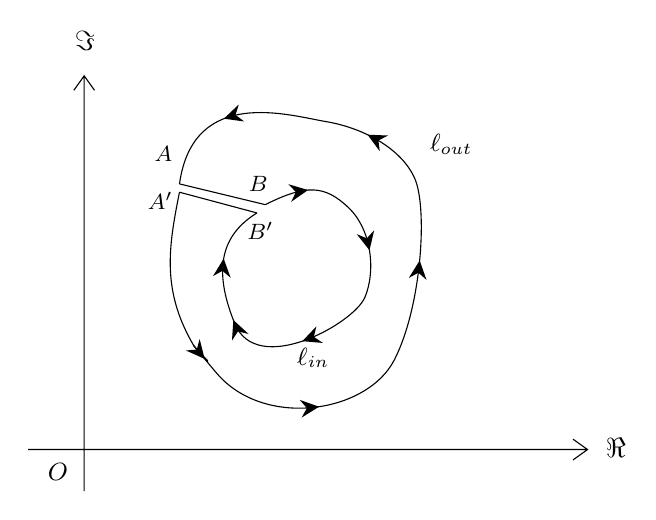
\begin{tikzpicture}[x=0.75pt,y=0.75pt,yscale=-1,xscale=1]
%uncomment if require: \path (0,300); %set diagram left start at 0, and has height of 300

%Shape: Axis 2D [id:dp04611299520330148] 
\draw  (107,219.06) -- (376.47,219.06)(133.95,39) -- (133.95,239.07) (369.47,214.06) -- (376.47,219.06) -- (369.47,224.06) (128.95,46) -- (133.95,39) -- (138.95,46)  ;
%Curve Lines [id:da4408212979573587] 
\draw    (179.87,91.07) .. controls (186.53,43.73) and (232.62,58.07) .. (250.53,61.07) .. controls (268.45,64.07) and (286.87,74.07) .. (293.2,88.4) .. controls (299.53,102.73) and (296.53,150.4) .. (283.33,175.97) .. controls (270.13,201.54) and (220.5,209.23) .. (197.65,182.12) .. controls (174.81,155.01) and (194.63,178.2) .. (193.33,175.97) ;
\draw [shift={(201.24,59.65)}, rotate = 342.17] [fill={rgb, 255:red, 0; green, 0; blue, 0 }  ][line width=0.08]  [draw opacity=0] (8.93,-4.29) -- (0,0) -- (8.93,4.29) -- (5.93,0) -- cycle    ;
\draw [shift={(270.48,67.37)}, rotate = 27.92] [fill={rgb, 255:red, 0; green, 0; blue, 0 }  ][line width=0.08]  [draw opacity=0] (8.93,-4.29) -- (0,0) -- (8.93,4.29) -- (5.93,0) -- cycle    ;
\draw [shift={(295.59,127.97)}, rotate = 96.21] [fill={rgb, 255:red, 0; green, 0; blue, 0 }  ][line width=0.08]  [draw opacity=0] (8.93,-4.29) -- (0,0) -- (8.93,4.29) -- (5.93,0) -- cycle    ;
\draw [shift={(247.14,198.42)}, rotate = 173.71] [fill={rgb, 255:red, 0; green, 0; blue, 0 }  ][line width=0.08]  [draw opacity=0] (8.93,-4.29) -- (0,0) -- (8.93,4.29) -- (5.93,0) -- cycle    ;
\draw [shift={(192.02,175.42)}, rotate = 230.07] [fill={rgb, 255:red, 0; green, 0; blue, 0 }  ][line width=0.08]  [draw opacity=0] (8.93,-4.29) -- (0,0) -- (8.93,4.29) -- (5.93,0) -- cycle    ;
%Straight Lines [id:da2752936846063838] 
\draw    (179.87,91.07) -- (221.2,101.07) ;
%Curve Lines [id:da2227786948358368] 
\draw    (221.2,101.07) .. controls (241.2,91.07) and (249.87,91.73) .. (261.2,102.4) .. controls (272.53,113.07) and (274.53,133.07) .. (269.2,145.73) .. controls (263.87,158.4) and (217.2,184.4) .. (206.53,158.4) .. controls (206.05,157.22) and (205.59,156.05) .. (205.17,154.91) .. controls (196.26,130.89) and (200.66,115.25) .. (217.2,105.07) ;
\draw [shift={(241.83,94.03)}, rotate = 170.78] [fill={rgb, 255:red, 0; green, 0; blue, 0 }  ][line width=0.08]  [draw opacity=0] (8.93,-4.29) -- (0,0) -- (8.93,4.29) -- (5.93,0) -- cycle    ;
\draw [shift={(271.41,123.08)}, rotate = 257.51] [fill={rgb, 255:red, 0; green, 0; blue, 0 }  ][line width=0.08]  [draw opacity=0] (8.93,-4.29) -- (0,0) -- (8.93,4.29) -- (5.93,0) -- cycle    ;
\draw [shift={(239.05,166.85)}, rotate = 339.24] [fill={rgb, 255:red, 0; green, 0; blue, 0 }  ][line width=0.08]  [draw opacity=0] (8.93,-4.29) -- (0,0) -- (8.93,4.29) -- (5.93,0) -- cycle    ;
\draw [shift={(205.83,156.66)}, rotate = 68.16] [fill={rgb, 255:red, 0; green, 0; blue, 0 }  ][line width=0.08]  [draw opacity=0] (8.93,-4.29) -- (0,0) -- (8.93,4.29) -- (5.93,0) -- cycle    ;
\draw [shift={(201.16,127.05)}, rotate = 95.63] [fill={rgb, 255:red, 0; green, 0; blue, 0 }  ][line width=0.08]  [draw opacity=0] (8.93,-4.29) -- (0,0) -- (8.93,4.29) -- (5.93,0) -- cycle    ;
%Straight Lines [id:da5896769090029934] 
\draw    (179.87,95.07) -- (217.2,105.07) ;
%Curve Lines [id:da07734592378285976] 
\draw    (187.2,169.73) .. controls (171.07,142.83) and (174.53,121.73) .. (179.87,95.07) ;

% Text Node
\draw (115.17,224.57) node [anchor=north west][inner sep=0.75pt]  [font=\small]  {$O$};
% Text Node
\draw (299.33,66.07) node [anchor=north west][inner sep=0.75pt]  [font=\small]  {$\ell _{out}$};
% Text Node
\draw (166.67,71.73) node [anchor=north west][inner sep=0.75pt]  [font=\footnotesize]  {$A$};
% Text Node
\draw (211.33,108.4) node [anchor=north west][inner sep=0.75pt]  [font=\footnotesize]  {$B'$};
% Text Node
\draw (212,86.4) node [anchor=north west][inner sep=0.75pt]  [font=\footnotesize]  {$B$};
% Text Node
\draw (163.33,93.73) node [anchor=north west][inner sep=0.75pt]  [font=\footnotesize]  {$A'$};
% Text Node
\draw (235.33,168.73) node [anchor=north west][inner sep=0.75pt]  [font=\small]  {$\ell _{in}$};
% Text Node
\draw (128.17,16.07) node [anchor=north west][inner sep=0.75pt]    {$\Im $};
% Text Node
\draw (384,212.4) node [anchor=north west][inner sep=0.75pt]    {$\Re $};


\end{tikzpicture}

    \caption{复杂路径示意图。}
    \label{fig:complexregion}
\end{figure}
由于$\ell_{in}$和$\ell_{out}$与割线$AB,A'B'$组成了闭合回路,根据柯西定理,我们有
\[
    \left[ \oint _{\ell_{out}} + \int _{\ell_{AB}} + \oint _{\ell_{in}} + \int _{\ell_{B'A'}} \right] f(z) dz = 0 \textrm{。}
\]   
由于割线$AB$与$A'B'$可以无限接近,可以看出二者方向相反,这两项互相抵消。于是我们有
\[
    \left[ \oint _{\ell_{out}} + \oint _{\ell_{in}}  \right] f(z) dz = 0,
\]
即
\[
    \oint_{\ell_{out}} f(z) dz = - \oint _{\ell_{in}}f(z) dz \textrm{。}
\]
若用逆时针方向积分表示,并考虑多个内边界$\ell_{i}$,我们有
\begin{equation}
    \ointctrclockwise_{\ell_{out}} f(z) dz = \sum_{i=1}^{n} \ointctrclockwise_{\ell_{i}} f(z) dz \textrm{。}
\end{equation}
就是说,外边界逆时针方向积分等于所有内边界逆时针方向积分之和。只要积分起点和终点固定,当积分路径连续变形时(即不跳过奇点),函数的积分值不变。

下面给出一个重要的例题。
\begin{examplebox}{计算积分\[ I = \oint_\ell (z-\alpha)^n dz, \]其中$n$为整数。}
首先,有柯西定理易知,若回路$\ell$不包含$\alpha$,则被积函数在$\ell$所围区域上是解析的,故积分值为零。下面讨论$\ell$包围$\alpha$的情形。
如果$n\geq 0$,被积函数在$\ell$所围区域是解析的,积分为零。若$n<0$,则有一个奇点$\alpha$。取以$\alpha$为圆心半径为$R$的圆周$C$,$R$大小任意。
于是圆周上有$z-\alpha = Re^{\imath \theta}$.
\begin{equation}
\begin{aligned}
    I &= \oint_\ell (z-\alpha)^n dz\\
     &= \oint_c R^n e^{\imath n \theta} d (\alpha + R e^{\imath \theta})\\
     & =  \imath R^{n+1} \int_0^{2\pi} e^{\imath (n+1)\theta}  d\theta \\
     & = 0 \quad \textrm{if} \quad n\neq -1.
\end{aligned}
\end{equation}
当$n = -1$时, $I = 2\pi \imath$。其实,从原函数的角度来看,这个结果很容易理解。当$n\neq -1$,原函数为$(z-\alpha)^{n+1}/(n+1)$, 绕$\alpha$一周
原函数变化量为零。而当$n=-1$时,原函数时$\ln(z-\alpha)$, 绕一周变化量为$2\pi \imath$。因此我们得到了非常重要的表达式
\begin{equation}
    \begin{aligned}
        & \frac{1}{2 \pi \mathrm{i}} \oint_l \frac{\mathrm{d} z}{z-\alpha}= \begin{cases}0 & (l \text { 不包围 } \alpha), \\
        1 & (l \text { 包围 } \alpha) \textrm{。} \end{cases} \\
        & \frac{1}{2 \pi \mathrm{i}} \oint_l(z-\alpha)^n \mathrm{~d} z=0 \quad(n \neq-1) \textrm{。}
        \end{aligned}
\end{equation}
\end{examplebox}
% \subsection{柯西积分公式}
% \section{留数定理}
% \label{sec:residual_theorem}
% \subsection{留数定理}
\label{subsec:residual_theorem}
柯西定理指出,若被积函数$f(z)$在回路$\ell$所围区域是解析的,则回路积分$\oint_\ell f(z) dz$为零.下面讨论所围区域包含奇点的情况.
假设一个含有$m$阶极点$z=z_0$的函数,它可以展开为洛朗级数
\[
  f(z) = \sum_{k = -m} ^{\infty} a_k (z - z_0)^k  
\]
取圆环内包含$z_0$的闭合回路,由柯西定理可知,回路积分$\oint_\ell f(z) dz = \oint_C f(z) dz$, 将洛朗展开带入逐项积分,可得
\[
\oint_\ell f(z) dz = \sum_{k = -m} ^{\infty} \oint_C  (z - z_0)^k dz,
\]
由前面例题可知,只有$a_{-1}$项不为零,其他项为零.而$a_{-1}$项的积分为$2\pi\imath$.因此,我们得到
\begin{equation}
    \oint_\ell f(z) dz = 2\pi \imath a_{-1} .
\end{equation}
又因为$a_{-1}$为函数$f(z)$在$z=z_0$处的留数,记为$Res f(z_0)$.于是有
\begin{equation}
    \oint_\ell f(z) dz = 2\pi \imath Res f(z_0) .
\end{equation}
扩展到多个奇点的情况,不难得到
\begin{equation}
    \oint_\ell f(z) dz = 2\pi \imath \sum_{j=1}^{n} Res f(z_j) .
\end{equation}
上式为\textbf{留数定理}的数学表达式,即回路积分可以写成被积函数在回路所围区域上各个奇点的留数之和.

下面介绍一下计算留数的一种方法.
通常,我们并不总是要将一个函数展开为洛朗级数来找出$a_{-1}$的值.如果$f(z)$有
$n$阶极点$z_0$,那么有
\begin{equation}
    \left(z-z_0\right)^n f(z)=a_{-n}+\cdots+a_{-1}\left(z-z_0\right)^{n-1}+a_0\left(z-z_0\right)^n+\cdots .
\end{equation}
不断求导后可以验证
\begin{equation}
    a_{-1}=\frac{1}{(n-1) !} \lim _{z \to z_0}\left[\frac{d^{n-1}}{d z^{n-1}}\left(\left(z-z_0\right)^n f(z)\right)\right]
\end{equation}
若 $f(z)$ 可以表示为 $P(z) / Q(z)$ 的特殊形式, 其中 $P(z)$ 和 $Q(z)$ 都在 $z_0$ 点 解析, $z_0$ 是 $Q(z)$ 的一阶零点. $P\left(z_0\right) \neq 0$, 从而 $z_0$ 是 $f(z)$ 的一阶极点, 则
\begin{equation}
    Res f\left(z_0\right)=\lim _{z \to z_0}\left(z-z_0\right) \frac{P(z)}{Q(z)}=\frac{P\left(z_0\right)}{Q^{\prime}\left(z_0\right)} .
\end{equation}
上式最后一步应用了罗毕达法则.
下面给出一些计算留数的例子.
\begin{examplebox}{计算留数.}
    
    \begin{enumerate}
        \item $\frac{1}{\sin z}$在$z=0$处的留数为$\lim_{z\to 0} \frac{z}{\sin{z}} = 1$.
        \item $\frac{\ln{z}}{z^2 + 4}$在$z=2e^{\imath \pi}$处的留数为$\lim_{z\to 2e^{\imath \pi}} \frac{(z-2e^{\imath \pi})\ln{z} }{z^2 + 4} = 
        \frac{\ln 2 + \imath \pi}{4\imath} = \frac{\pi}{4} - \frac{\imath\ln{2}}{4}.$
        \item $f(z) = \frac{\cot{\pi z}}{z(z+2)}$在$z=0$处的留数.\\
            \[
              f(z) = \frac{1}{z} \left[\frac{1}{\pi z} + O(z) \right]\frac{1}{2} \left[1 - \frac{z}{2} + O(z^2)\right]  
            \]
            可以得到该函数的留数为$-1/(4\pi)$.
        \item $f(z) = \frac{1}{z^n - 1}$在$z=1$处的留数可通过如下方法.可知
        \[
            f(z)=\frac{1}{z^n-1}=\frac{1}{(z-1)\left(z^{n-1}+z^{n-2}+\cdots+z+1\right)},
        \]
        因此,有
        \[
            \begin{aligned}
                \operatorname{Res} f(1) & =\lim _{z \to 1}\left[(z-1) \frac{1}{(z-1)\left(z^{n-1}+z^{n-2}+\cdots+z+1\right)}\right] \\
                & =\lim _{z \to 1} \frac{1}{z^{n-1}+z^{n-2}+\cdots+z+1}=\frac{1}{n} .
            \end{aligned}
        \]
        或者用 $$
        \lim _{z \to 1}\left[\frac{1}{\left(z^n-1\right)^{\prime}}\right]=\lim _{z \to 1} \frac{1}{n z^{n-1}}=\frac{1}{n} .
        $$ 因此,此函数在$z=1$处的留数为$1/n$.
    \end{enumerate}
\end{examplebox}


% \subsection{留数定理的应用}
% \label{subsec:residual_theorem_applications}

% \section{}